\section{Frequency Exploitation}

%%%%%%%%%%%%%%%%%%%%%%%%%%%%%%%%%%%%%%%%%%%%%%%%%%%%%%%%%%%%

\subsection{Spatial Domain and Frequency Domain}
An image can be represented in two fundamental ways: the spatial domain and the frequency domain. In the \textbf{spatial domain}, an image is described as a matrix of pixel intensity values, where each value corresponds to the brightness of a pixel at a specific location. Spatial domain methods process images based on the direct manipulation of these pixel values \cite{gonzalez2002digital}. Common operations in the spatial domain include contrast enhancement, smoothing, sharpening, and edge detection. These operations use filters or kernels that are convolved directly with the image matrix.\\\\
In contrast, the \textbf{frequency domain} represents an image as a sum of sinusoids of varying frequencies and amplitudes, obtained by applying a transformation such as the Discrete Fourier Transform (DFT) or Discrete Cosine Transform (DCT) \cite{bracewell1986fourier}. The frequency domain reveals how pixel values change across the image, with low frequencies representing smooth areas and high frequencies representing sharp edges and fine details. Frequency domain methods are particularly useful for tasks like image compression and noise reduction.\\\\
The transformation from spatial domain to frequency domain is often done using the 2D Fourier Transform. This transform decomposes the image into its sinusoidal components, which can be analyzed, modified, or truncated for various applications. The inverse transform reconstructs the image back into the spatial domain. For example, JPEG image compression uses the DCT to transform image blocks into frequency components, discards high-frequency data that is less perceptible to the human eye, and stores the remaining information efficiently \cite{wallace1992jpeg}.
\begin{figure}[hbt]
    \centering
    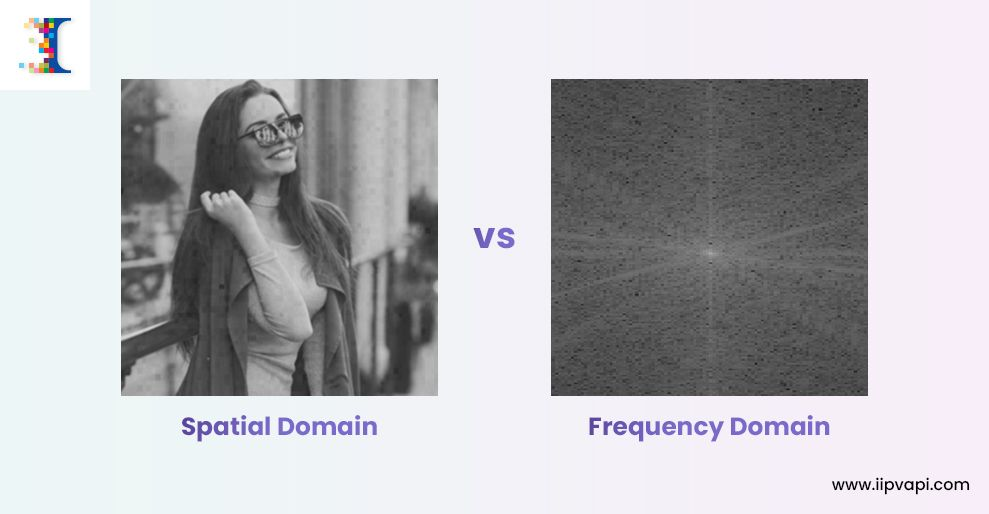
\includegraphics[width=0.8\textwidth]{theoretical-background/image/frequency-vs-spatial.jpg}
    \caption{Comparison between spatial and frequency domain representations of an image}
    \label{fig:freq_and_space}
\end{figure}

\textbf{2D Discrete Fourier Transform (DFT)}: It converts an image from the spatial domain to the frequency domain. Given an image of size $M \times N$, the DFT is defined as:
\begin{align}
    F(u,v) = \sum_{x=0}^{M-1} \sum_{y=0}^{N-1} f(x,y) e^{-j 2\pi \left(\frac{ux}{M} + \frac{vy}{N}\right)}
\end{align}

\textbf{Inverse 2D Discrete Fourier Transform (IDFT)}: This reconstructs the image back into the spatial domain:
\begin{align}
    f(x,y) = \frac{1}{MN} \sum_{u=0}^{M-1} \sum_{v=0}^{N-1} F(u,v) e^{j 2\pi \left(\frac{ux}{M} + \frac{vy}{N}\right)}
\end{align}

\textbf{Filtering in Frequency Domain}: Many spatial filters can be implemented more efficiently in the frequency domain by multiplying the frequency representations instead of convolving in the spatial domain. This is enabled by the convolution theorem, which states that convolution in the spatial domain corresponds to multiplication in the frequency domain.

%%%%%%%%%%%%%%%%%%%%%%%%%%%%%%%%%%%%%%%%%%%%%%%%%%%%%%%%%%%%

% \subsection{Convolutional Neural Networks (CNN)}
% % Convolutional Neural Networks (CNNs) are a class of deep learning models that have become the foundation for many computer vision tasks, such as image classification, object detection, and segmentation. CNNs are specifically designed to process grid-like data, such as images, by leveraging the hierarchical pattern in images to automatically learn spatial hierarchies of features. The architecture of a CNN is composed of multiple layers, including convolutional layers, pooling layers, and fully connected layers, as shown in figure \ref{fig:cnn}. CNNs are particularly efficient in processing images due to their ability to capture local dependencies while maintaining translation invariance.

% In the early days of Computer Vision, most of the approaches focus on Feature Extraction using Un-Supervised Machine Learning combine with   classification such as SVM or Neutral Networks to classify the pictures labels, however, it is not possible for Segmentational and Object Detection due to the computational problems and feature extractions, take example for a 64x64x3 pictures, if we use traditional feature extractions, let assume it is 32x32x6 using PCA, then we have to input the total of 12288 Input Nodes, for this we want to consider for more, control-able ways and faster computations.

% Convolutional Neural Networks (CNNs) are a class of deep learning models specifically designed for processing data with a grid-like structure, such as images and time-series data. CNNs exploit the spatial and temporal hierarchies in data, making them highly effective for tasks like image recognition, object detection, and natural language processing. The core building block of a CNN is the \textit{convolution operation}, which applies a filter (or kernel) to an input to extract local patterns. Mathematically, for a 2D input \( I(x, y) \) and a kernel \( K(u, v) \),  in realistic application, the CNNs mostly contructed using cross-correlation, which is faster in computations time:

% \[
% S(x, y) = \sum_{u}\sum_{v} I(x + u, y + v) \cdot K(u, v)
% \]

% % The core component of a CNN is the Convolutional Layer, where a filter (or kernel) is convolved with the input image to extract features such as edges, textures, and patterns. The filter slides over the image with a specified stride, and the result of this convolution is passed through a non-linear activation function, typically the Rectified Linear Unit (ReLU) \cite{goodfellow2016deep}. This operation allows the network to detect low-level features in the early layers and more complex patterns in deeper layers.

% Following the convolutional layer, a Pooling Layer is often applied, which extracts the importance information of a regions of Feature Map. The most common pooling operation is max-pooling, where the maximum value from a region is selected, reducing the size of the feature map while preserving important information. This helps to make the model more invariant to small translations of the image.

% Finally, the fully connected layers at the end of the network help in classification by using the features extracted from the convolutional layers and pooling layers to make predictions. The last fully connected layer typically uses a softmax activation function for multi-class classification tasks.

% In summary, CNNs are a powerful class of models in deep learning that are particularly suited for image-related tasks due to their ability to learn hierarchical feature representations efficiently.

% \begin{figure}[hbt]
%     \centering
%     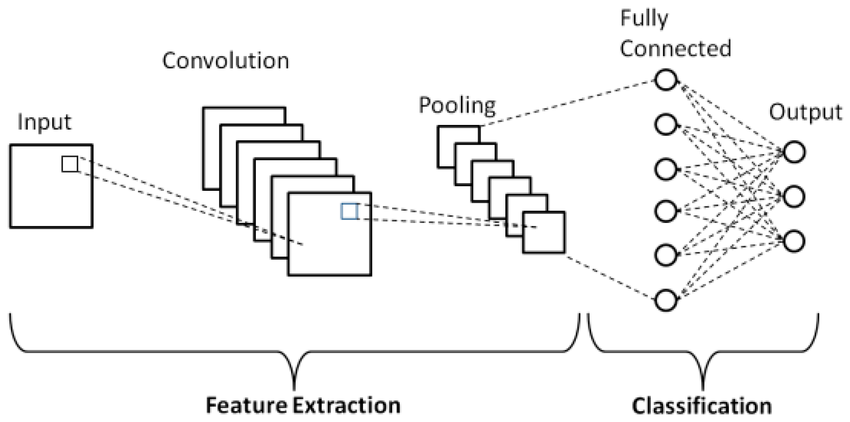
\includegraphics[width=1\textwidth]{theoretical-background/image/cnn.png}
%     \caption{Schematic diagram of a basic Convolutional Neural Network (CNN) architecture.}
%     \label{fig:cnn}
% \end{figure}


% % \textbf{Convolution Operation}: The convolution operation in CNNs is defined as follows. Given an input image $I$ and a filter $K$, the convolution operation produces an output feature map $O$. The output is calculated by taking the dot product between the filter and the image at each location as the filter slides over the image.

% % \begin{align}
% % O(i,j) = (I * K)(i,j) = \sum_m \sum_n I(i+m, j+n) \cdot K(m,n)
% % \end{align}

% \textbf{Max Pooling}: Max-pooling is used to reduce the spatial dimensions of the feature map by selecting the maximum value in a specified window, often $2 \times 2$. This operation helps to decrease the computational load while preserving the most important features.

% \begin{align}
% \text{MaxPool}(I) = \max(I)
% \end{align}

% \textbf{Fully Connected Layer}: After the convolution and pooling operations, the flattened output is passed through a fully connected layer. This layer is a standard neural network layer where each neuron is connected to every neuron in the previous layer. The output of this layer is typically passed through an activation function like softmax for classification tasks.

% \begin{align}
% FC(x) = W \cdot x + b
% \end{align}

% %%%%%%%%%%%%%%%%%%%%%%%%%%%%%%%%%%%%%%%%%%%%%%%%%%%%%%%%%%%%

% \subsection{Transformer}
% Transformer is a deep learning architecture showed in figure \ref{fig:transformer} that was introduced in 2017 by Vaswani et al \cite{NIPS2017_3f5ee243}. It builds on the ideas presented in two influential researchs, sequence to sequence \cite{NIPS2014_a14ac55a, DBLP:journals/corr/WuSCLNMKCGMKSJL16} and attention mechanism \cite{luong-etal-2015-effective}, and has become the state-of-the-art architecture for various natural language processing tasks.\\\\
% The Transformer Encoder is composed of multiple layers. The first layer is Multi-head Attention, and the second layer is Position-wise Feed-forward network. In the Encoder Self-Attention, Queries, Keys, and Values are all derived from the outputs of the previous Encoder Layer. Both sublayers use a residual connection, inspired by the ResNet architecture \cite{he2016deep}. This additional residual connection is immediately followed by Layer Normalization \cite{ba2016layer}. As a result, the Transformer Encoder produces a vector representation for each position of the input sequence.\\\\
% The Transformer Decoder is also a stack of multiple layers. In addition to the two sublayers described in the Encoder, the Decoder includes a third sublayer called the Encoder-Decoder Attention, or Cross-Attention, between these two. In the Encoder-Decoder Attention, Queries are derived from the outputs of the previous Decoder Layer, while the Keys and Values are derived from the Transformer Encoder outputs. In the Decoder Self-Attention, Queries, Keys, and Values are derived from the outputs of the previous Decoder Layer. However, each position in the Decoder can only attend to all positions in the Decoder up to that position, which is called Masked Self-Attention. This Masked Self-Attention preserves the autoregressive property, ensuring that the prediction only depends on those output tokens that have been generated.\\\\
% In summary, the transformer model is a powerful and flexible architecture that owes its success to the combination of the sequence to sequence learning approach and the attention mechanism.\\\\ 
% \begin{figure}[hbt]
%     \centering
    
%     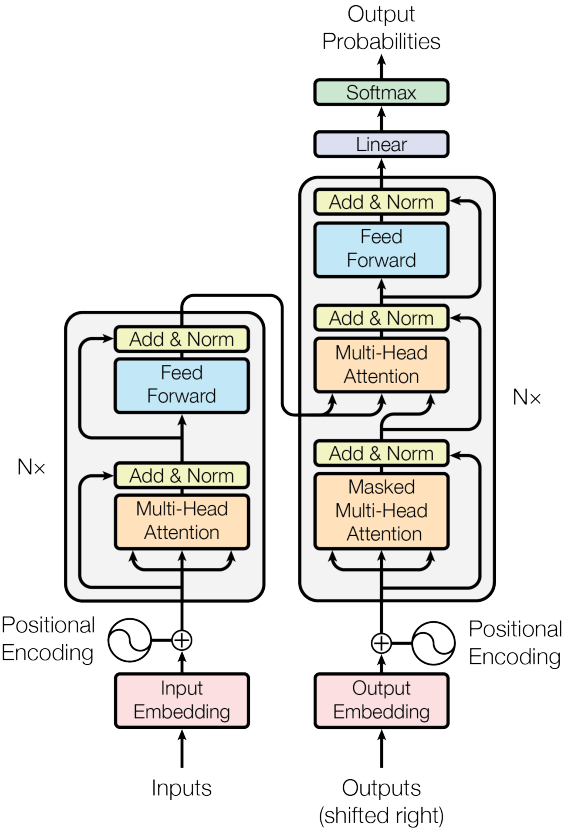
\includegraphics[width=0.6\textwidth]{theoretical-background/image/transformer.png}
%     \caption{The architecture of transformers presented in the research paper "Attention is all you need" \cite{NIPS2017_3f5ee243}}
%     \label{fig:transformer}
% \end{figure}
% \textbf{Scaled Dot-Product Attention}: It computes how much each value vector contributes to the output vector, based on the similarity between the query vector Q and the key vector Q. The similarity is measured by the dot product, which is scaled down by the square root of the dimension of the key vector $d_k$. The scaled dot products are then normalized by a softmax function to get the attention weights. The output vector is the weighted sum of the value vectors.
% \begin{align}
%     Attention (Q,K,V)=softmax(\frac{QK^T}{\sqrt(d_k)})V
% \end{align}

% \textbf{Multi-head Attention}: It applies the attention function multiple times in parallel, each of them is called a head, using different projections of the query, key and value vectors. This allows the model to capture different aspects of the input and output sequences. The outputs of the multi-head attention are concatenated and projected to get the final output.
% \begin{align}
%     MultiHead(Q,K,V)= Concat(head_1,...,head_h)W^O\\
%     \text{where } head_i=Attention(QW_{i}^Q, KW_{i}^K, VW_{i}^V)
% \end{align}

% \textbf{Position-wise Feed-forward Networks}: This is a way of transforming the output of the attention layers using a simple neural network that consists of two linear layers with a ReLU activation in between. The network is applied to each position separately and identically, meaning that it does not depend on the order of the sequence. The network has the same input and output dimension as the attention layers, but a larger hidden dimension.
% \begin{align}
%     FFN(x)=max(0,x\cdot W_1+b_1)\cdot W_2+b_2
% \end{align}

%%%%%%%%%%%%%%%%%%%%%%%%%%%%%%%%%%%%%%%%%%%%%%%%%%%%%%%%%%%%

\subsection{Wavelet Transform}
\textbf{Wavelet Transform (WT)} is a mathematical tool used for analyzing localized variations of signals in both time and frequency domains. Unlike the Fourier Transform, which only provides frequency information, WT offers multi-resolution analysis, capturing both coarse and fine-grained features of a signal. This is achieved by representing the signal in terms of shifted and scaled versions of a prototype function known as the \textit{mother wavelet} \cite{mallat1989theory}. WT is especially useful for analyzing non-stationary signals, where frequency components change over time.

The Continuous Wavelet Transform (CWT) of a signal $x(t)$ is defined as:
\begin{align}
    W(a, b) = \frac{1}{\sqrt{|a|}} \int_{-\infty}^{\infty} x(t) \psi^*\left(\frac{t - b}{a}\right) dt
\end{align}
where $a$ is the scale parameter, $b$ is the translation parameter, and $\psi(t)$ is the mother wavelet. The CWT produces a redundant and highly informative representation of the signal, making it suitable for detailed analysis but inefficient for storage and computation. To address these drawbacks, the Discrete Wavelet Transform (DWT) was introduced as an efficient and practical alternative.

\textbf{The Discrete Wavelet Transform (DWT)} is a mathematical technique used to decompose a signal into components at various frequency bands and resolutions. It was popularized by Daubechies in the early 1990s \cite{daubechies1992ten} and has become a cornerstone in signal and image processing, notably in compression, denoising, and feature extraction.

DWT applies a series of high-pass and low-pass filters to the input signal to extract both high-frequency (detail) and low-frequency (approximation) information. After each filtering step, the signal is downsampled by a factor of two. This process is recursively applied to the low-frequency component, creating a multi-resolution representation of the original signal, commonly referred to as a wavelet decomposition tree.\\

One of the main advantages of DWT over traditional Fourier Transform is its ability to provide both time and frequency localization. This means DWT can analyze transient, non-stationary, or time-varying signals more effectively. Moreover, DWT is highly efficient due to the use of compactly supported wavelets and the decimation process.\\

In image processing, 2D-DWT is performed by applying the DWT first to image rows and then to columns, resulting in four subbands: LL (approximation), LH (horizontal details), HL (vertical details), and HH (diagonal details). This hierarchical decomposition helps isolate different directional features and is widely used in image compression standards such as JPEG 2000 \cite{taubman2002jpeg2000}.

\begin{figure}[hbt]
    \centering
    
    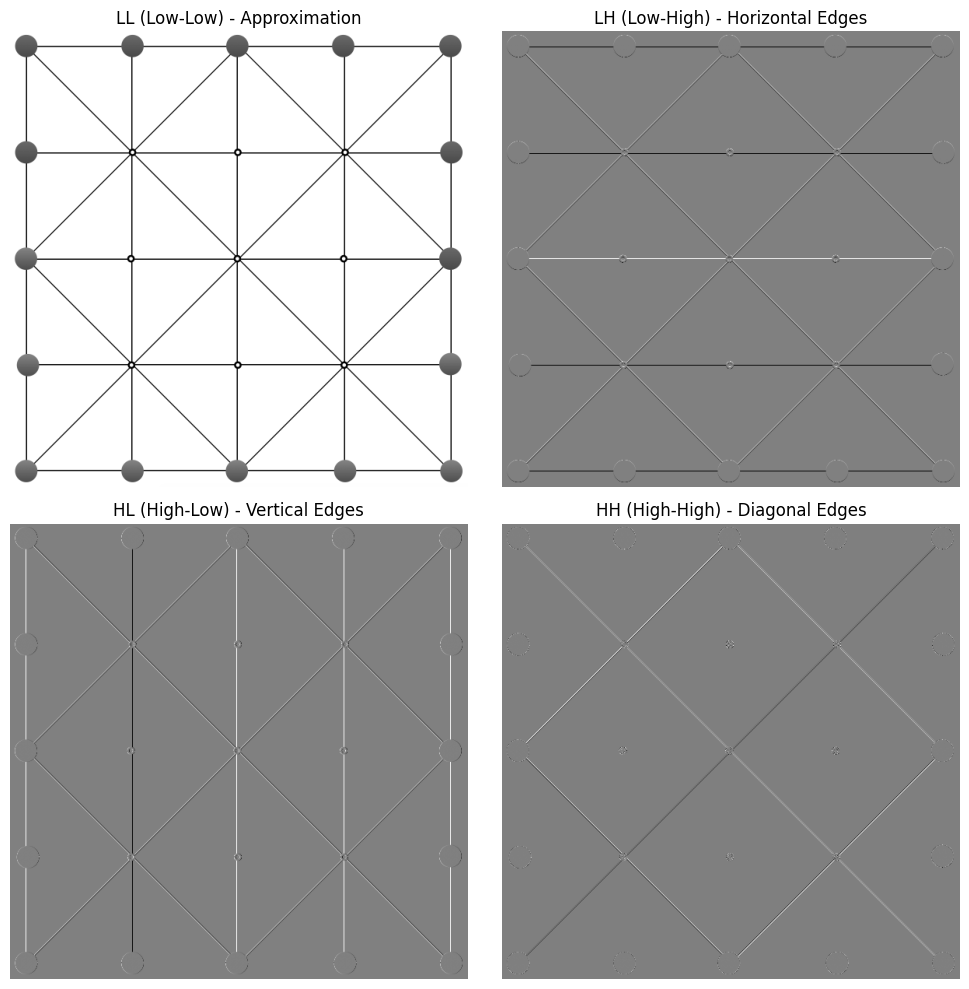
\includegraphics[width=0.5\textwidth]{theoretical-background/image/2D-DWT.png}
    \caption{Result of applying 2D-DWT once onto an image.}
    \label{fig:2D_DWT}
\end{figure}

\textbf{Scaling Function}: The DWT uses two fundamental functions: the mother wavelet $\psi(t)$ for capturing details, and the scaling function $\phi(t)$ for approximating the signal. The wavelet coefficients are computed as follows:
\begin{align}
    c_{j,k} = \int x(t) \phi_{j,k}(t) dt,\quad d_{j,k} = \int x(t) \psi_{j,k}(t) dt
\end{align}
where $j$ and $k$ represent scale and translation indices, respectively.

\textbf{Filter Bank Implementation}: DWT can be efficiently implemented using a two-channel filter bank:
\begin{itemize}
    \item \textit{Low-pass filter (scaling)}: Captures approximation coefficients.
    \item \textit{High-pass filter (wavelet)}: Captures detail coefficients.
\end{itemize}
Let $h[n]$ and $g[n]$ denote the low-pass and high-pass filters, respectively. Then:
\begin{align}
    a[n] &= \sum_{k} x[k] h[2n-k] \\
    d[n] &= \sum_{k} x[k] g[2n-k]
\end{align}
where $a[n]$ and $d[n]$ are the approximation and detail coefficients after one level of decomposition.
